%========================================================================
% Modelo para elaboracao de textos academicos: TCC, dissertacoes e teses
% Elaborado pelo GISIS - Grupo de Imageamento Sismico e Inversao Sismica.
%========================================================================
\chapter{Metodologia}
\label{ch:metodologia}

asdfasdf

\section{Construção dos modelos de velocidade}

\begin{figure}[H]
	\centering
	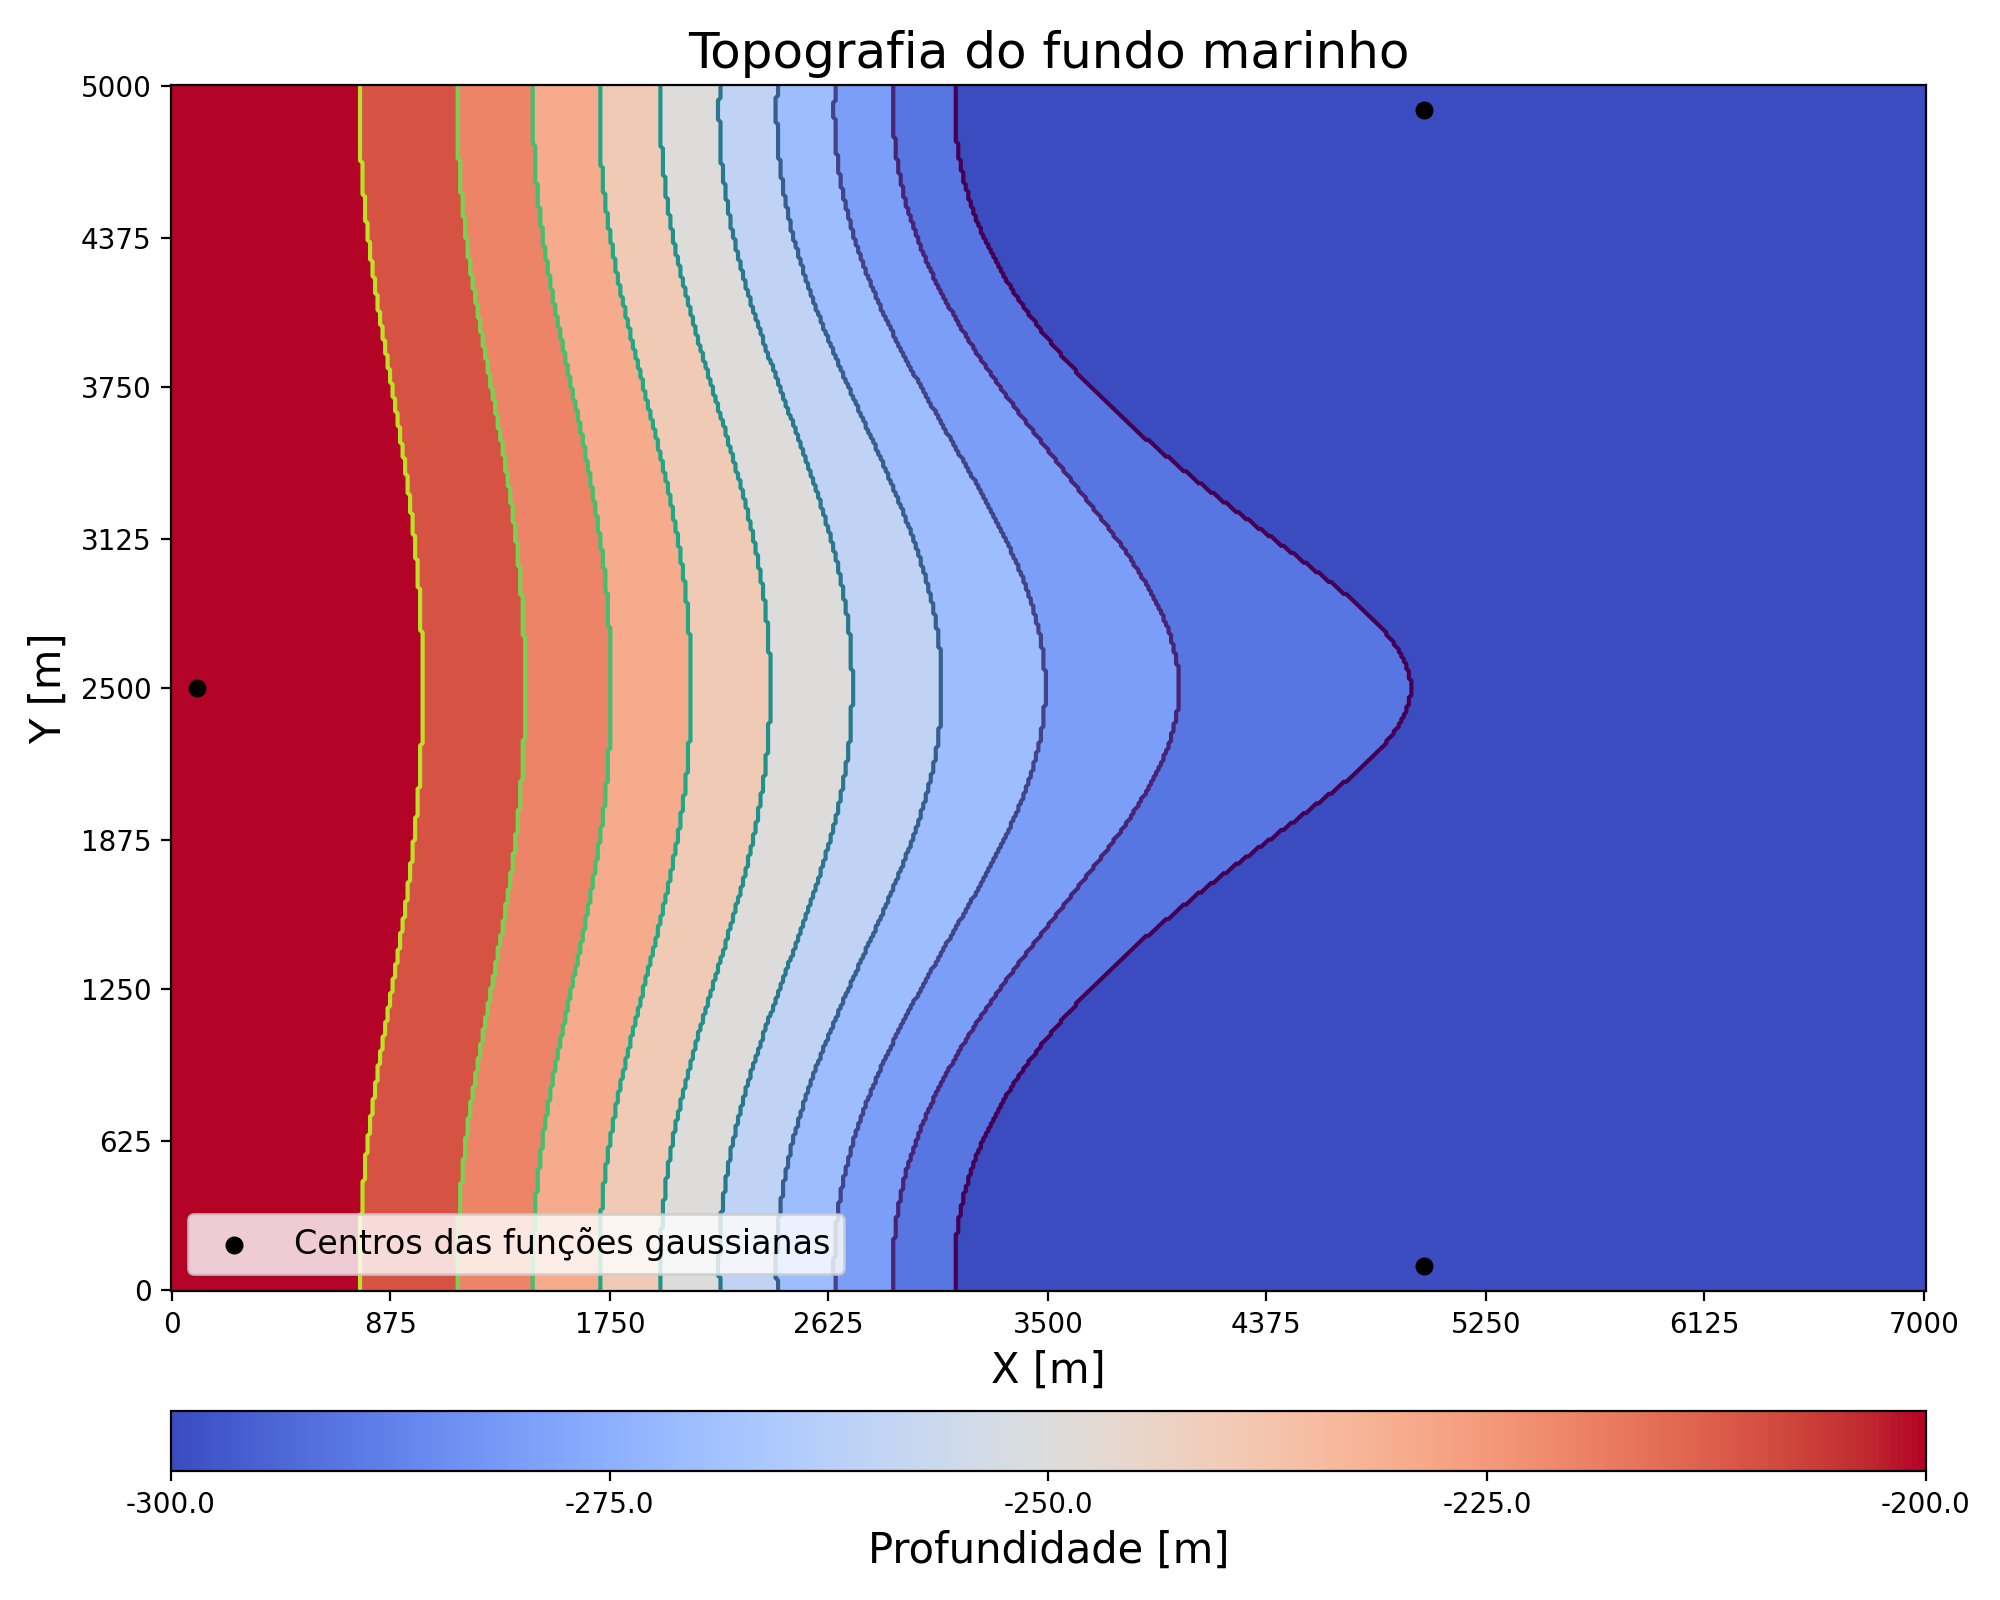
\includegraphics[width=11cm,height=8cm]{Imgs/Metodologia/water_bottom_surface_gaussian.png}
	\caption{caption}
	\label{fig:}	
\end{figure}


\begin{figure}[H]
	\centering
	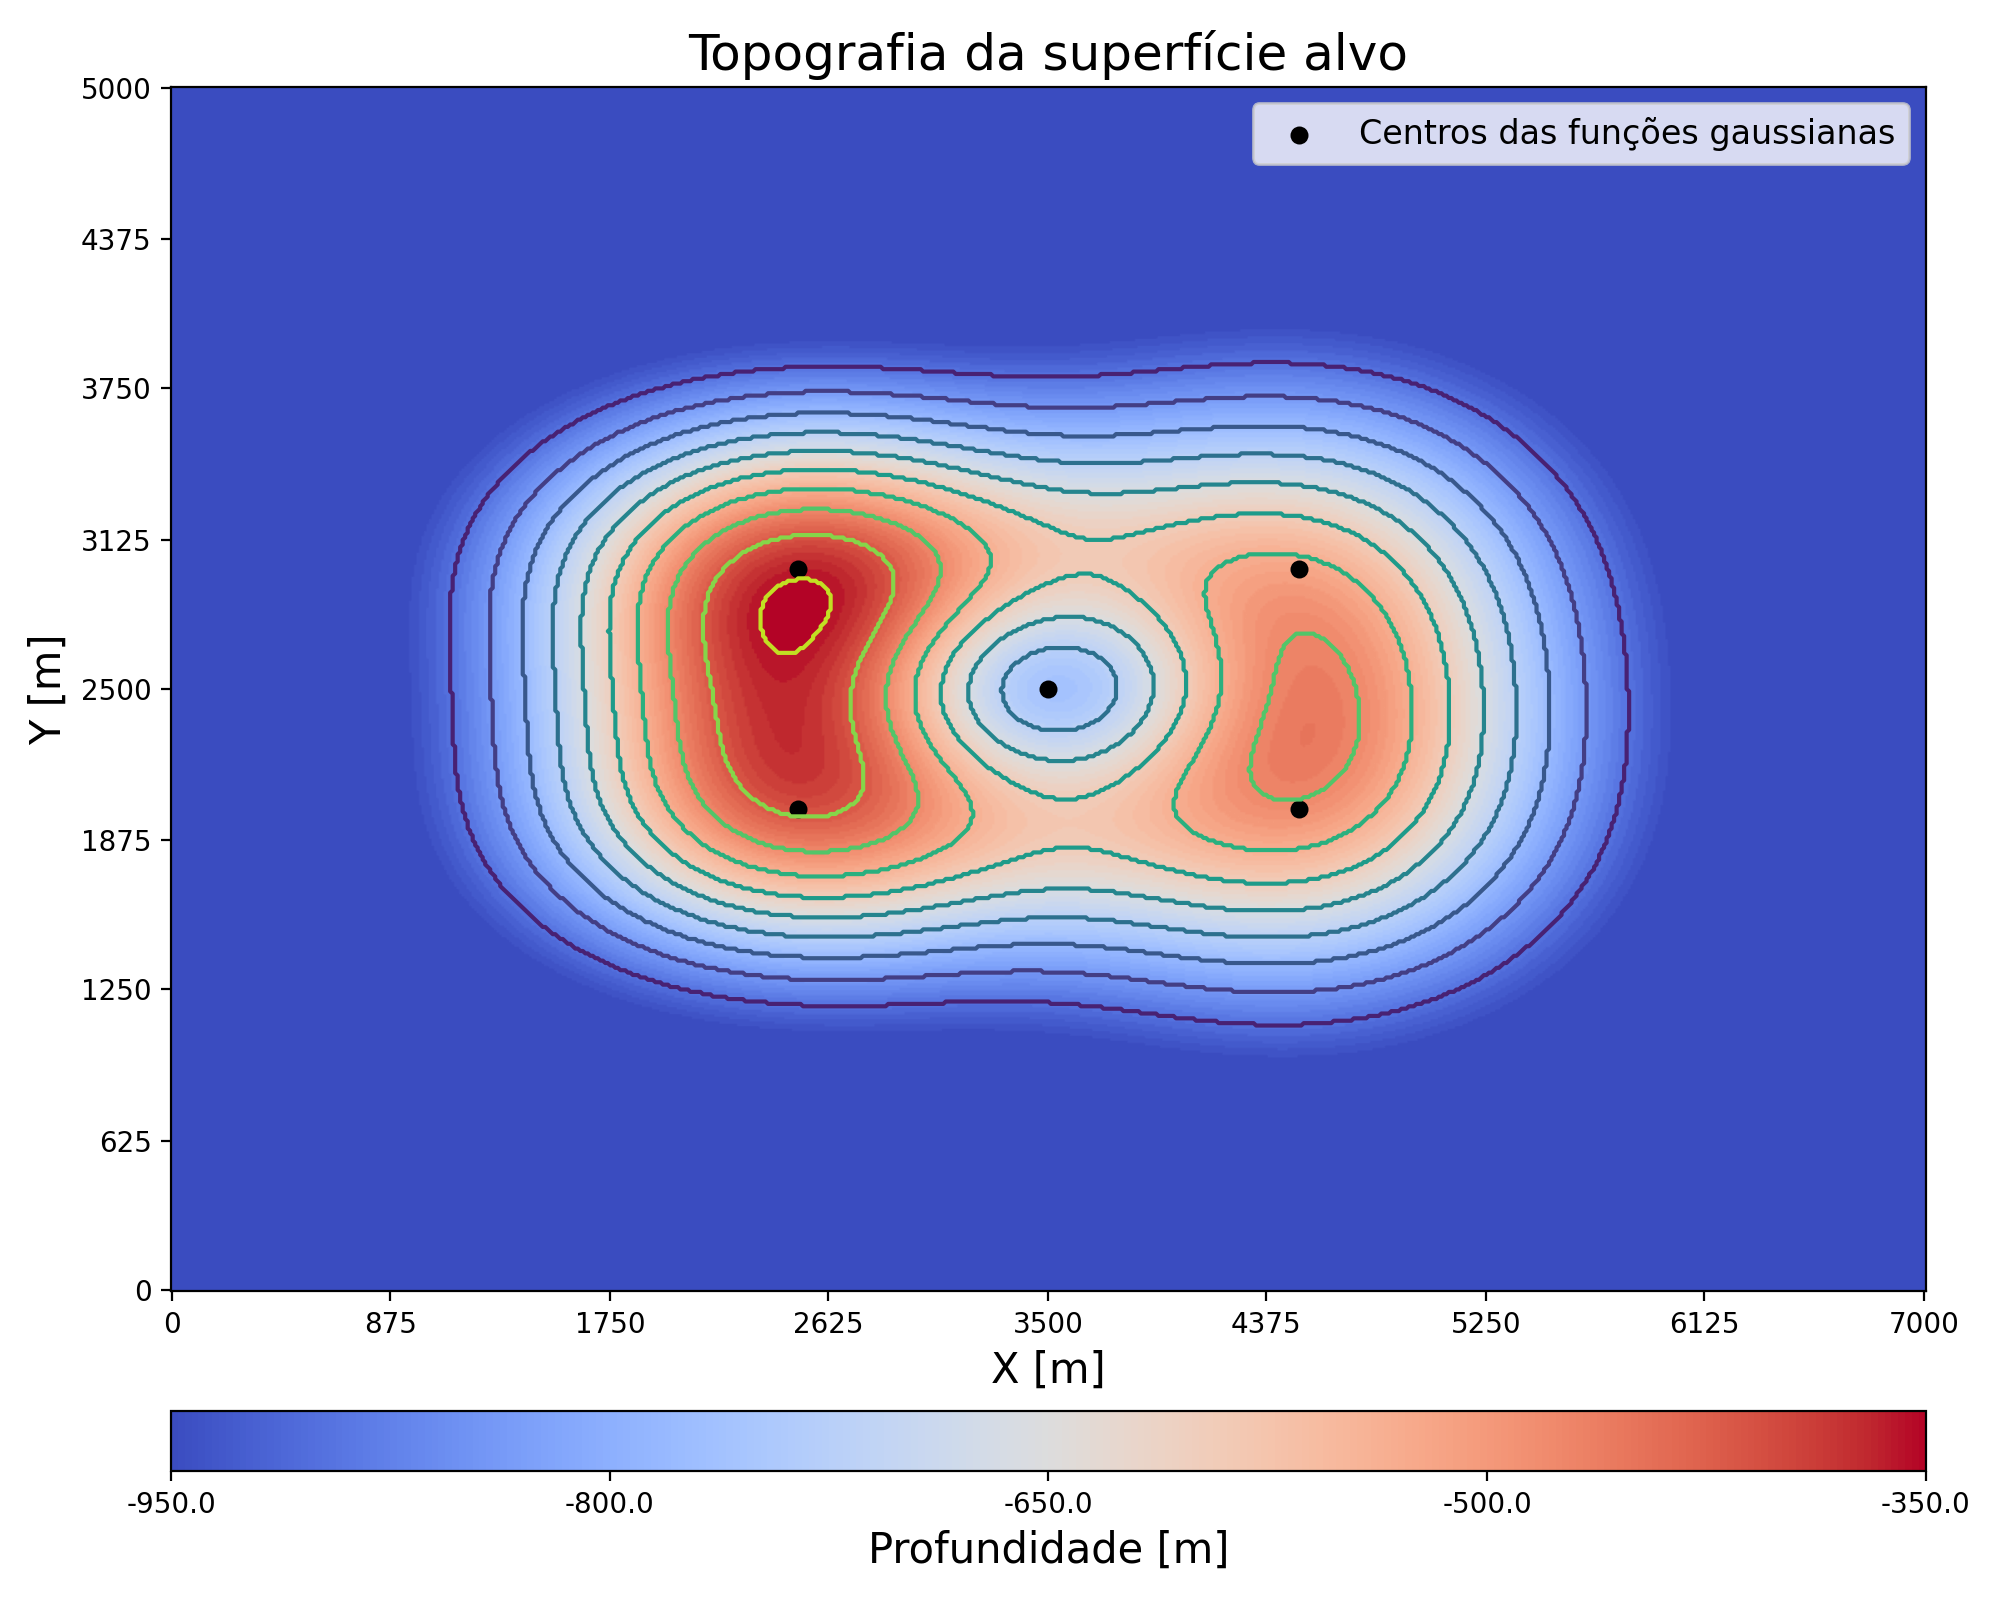
\includegraphics[width=11cm,height=8cm]{Imgs/Metodologia/target_surface_gaussian.png}
	\caption{caption}
	\label{fig:}	
\end{figure}


\begin{figure}[H]
	\centering
	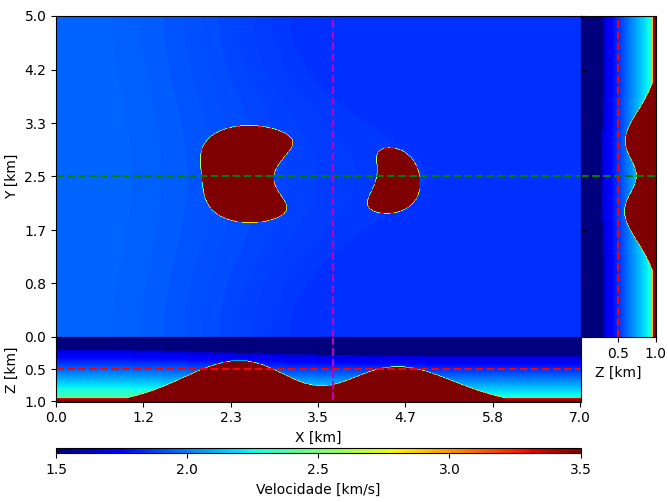
\includegraphics[width=12cm,height=9cm]{Imgs/Metodologia/true_model.png}
	\caption{caption}
	\label{fig:}	
\end{figure}


\begin{figure}[H]
	\centering
	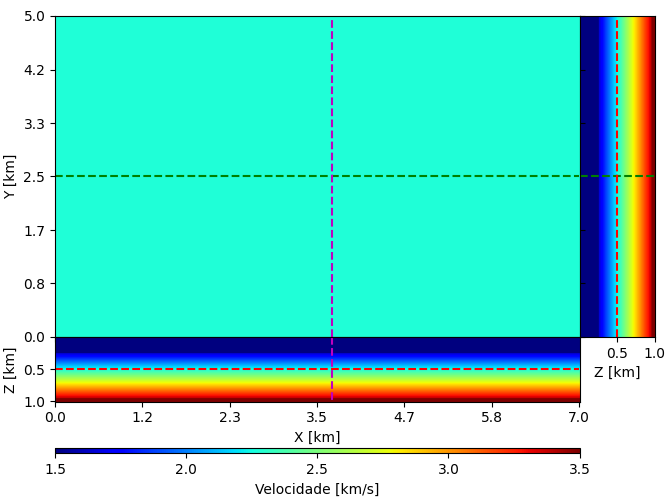
\includegraphics[width=12cm,height=9cm]{Imgs/Metodologia/init_model.png}
	\caption{caption}
	\label{fig:}	
\end{figure}




\section{Geometria de aquisição}

\begin{figure}[H]
	\centering
	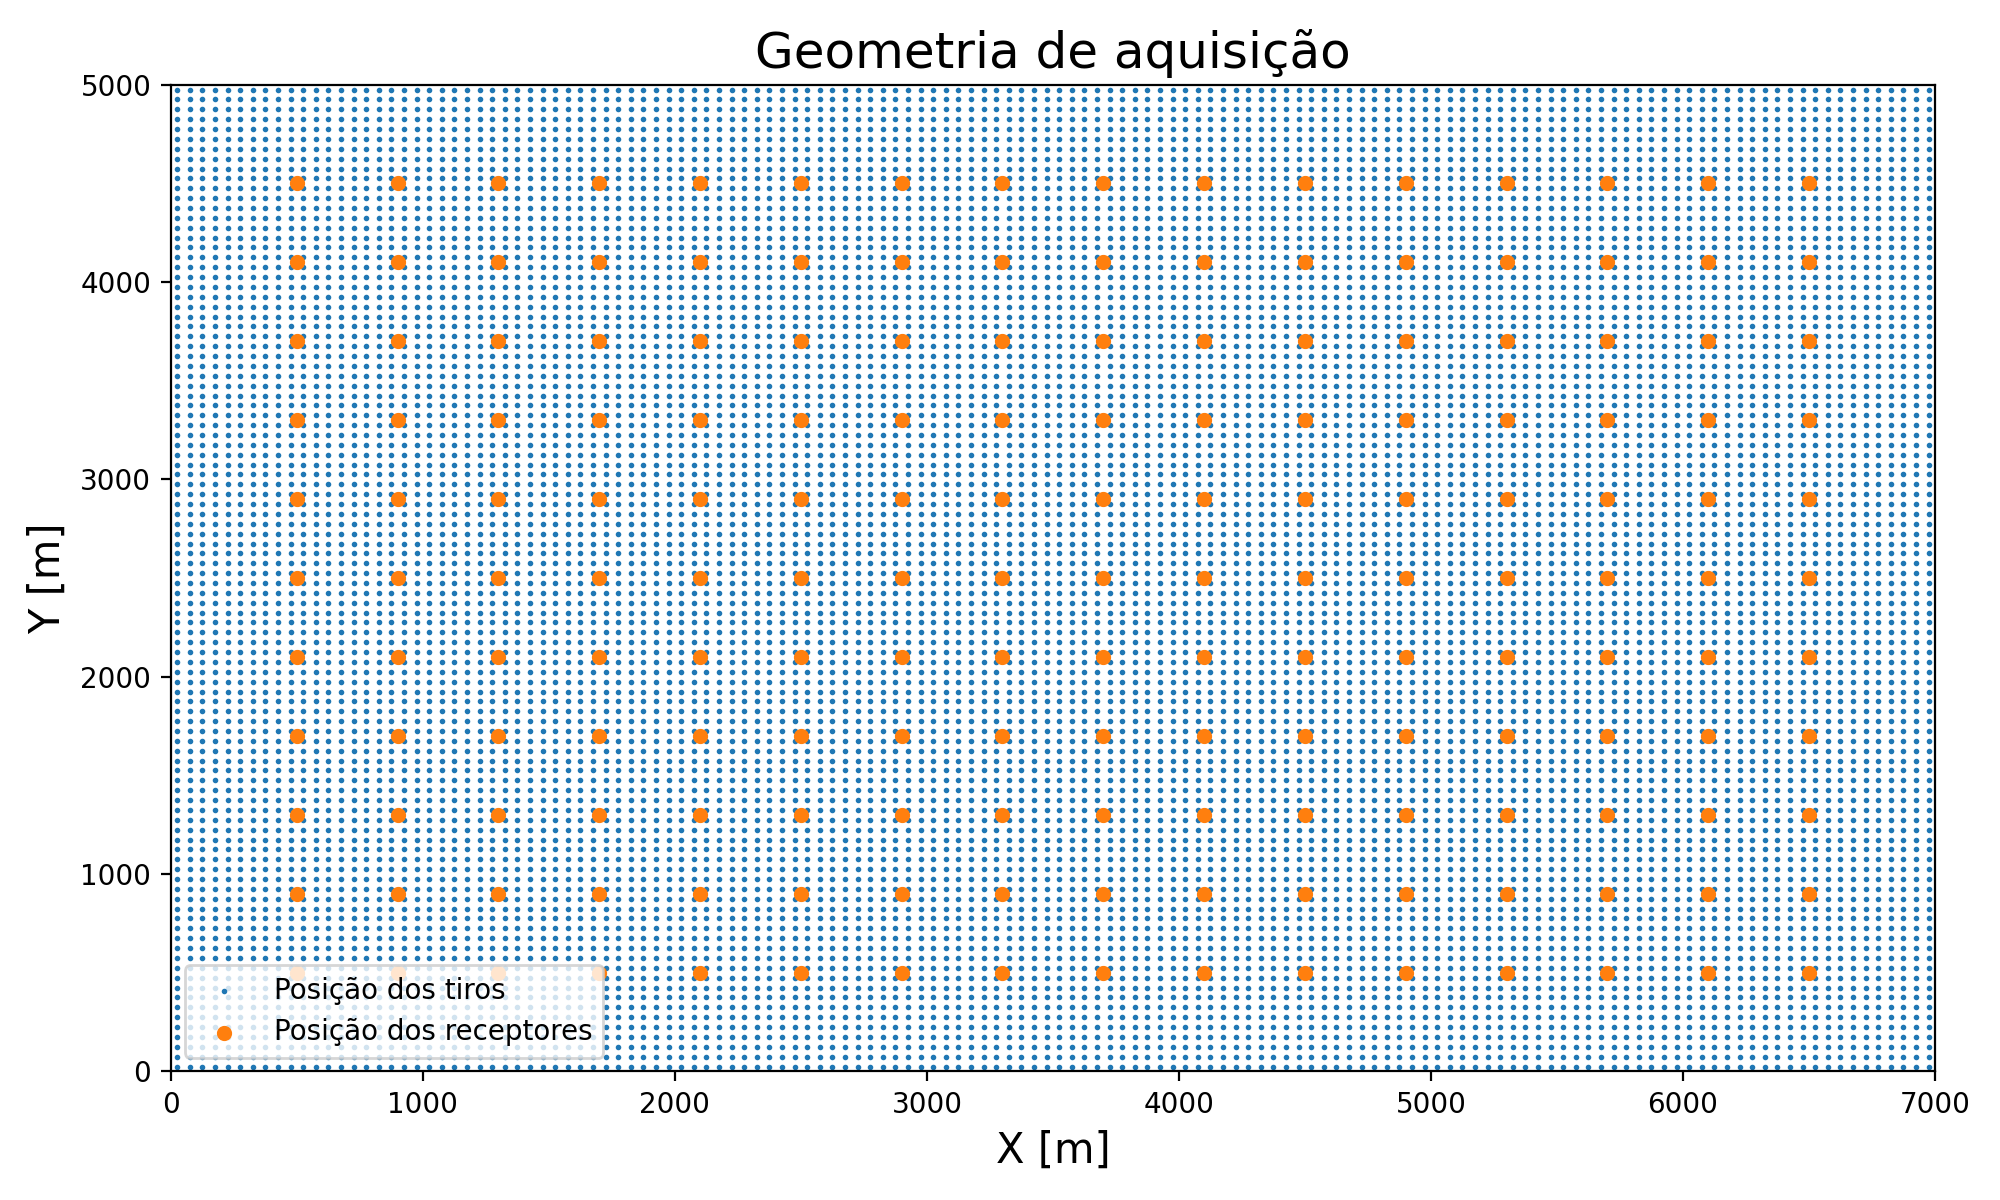
\includegraphics[width=12cm,height=7cm]{Imgs/Metodologia/complete_geometry.png}
	\caption{caption}
	\label{fig:}	
\end{figure}


\begin{figure}[H]
	\centering
	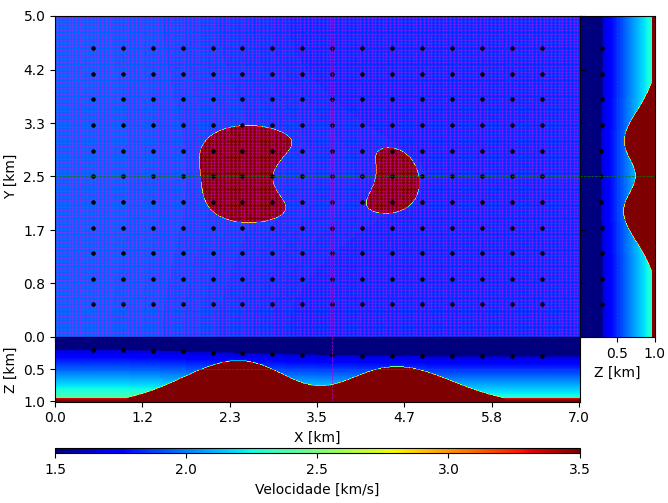
\includegraphics[width=12cm,height=9cm]{Imgs/Metodologia/true_model_geometry.png}
	\caption{caption}
	\label{fig:}	
\end{figure}


\begin{figure}[H]
	\centering
	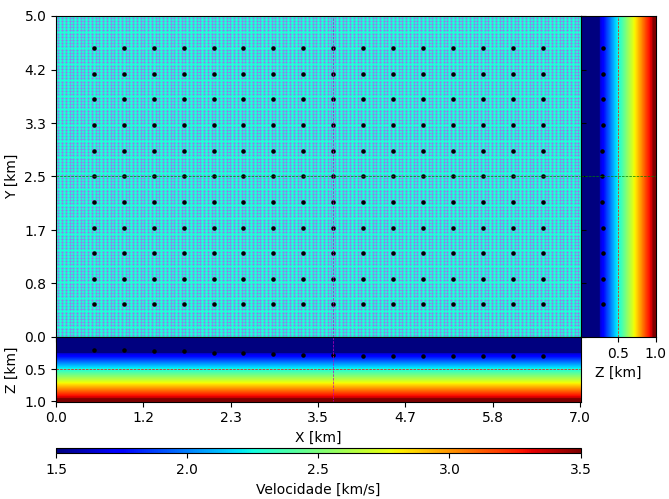
\includegraphics[width=12cm,height=9cm]{Imgs/Metodologia/init_model_geometry.png}
	\caption{caption}
	\label{fig:}	
\end{figure}




\section{Dado observado sintético}


\begin{figure}[H]
	\centering
	\subfloat[]{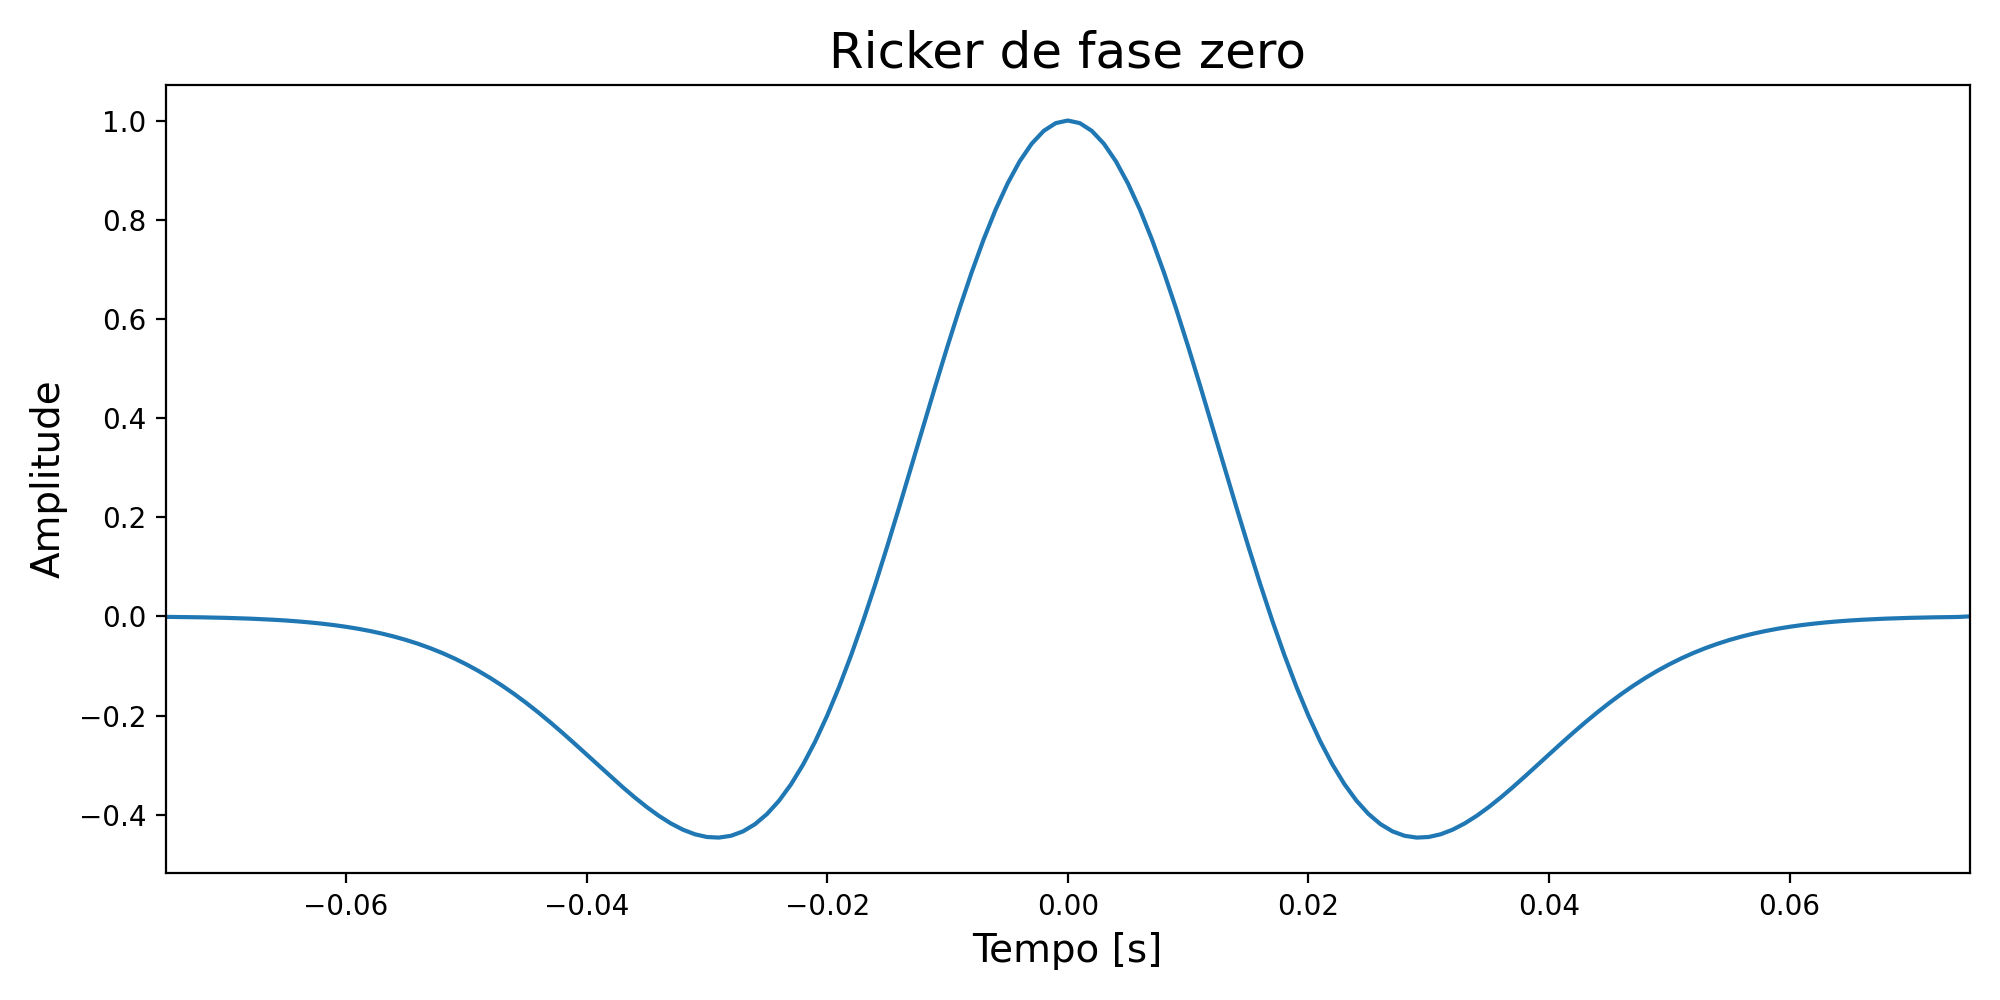
\includegraphics[width=8cm,height=4cm]{Imgs/Metodologia/ricker_zero_phase_a.png}\label{fig:}}
	\subfloat[]{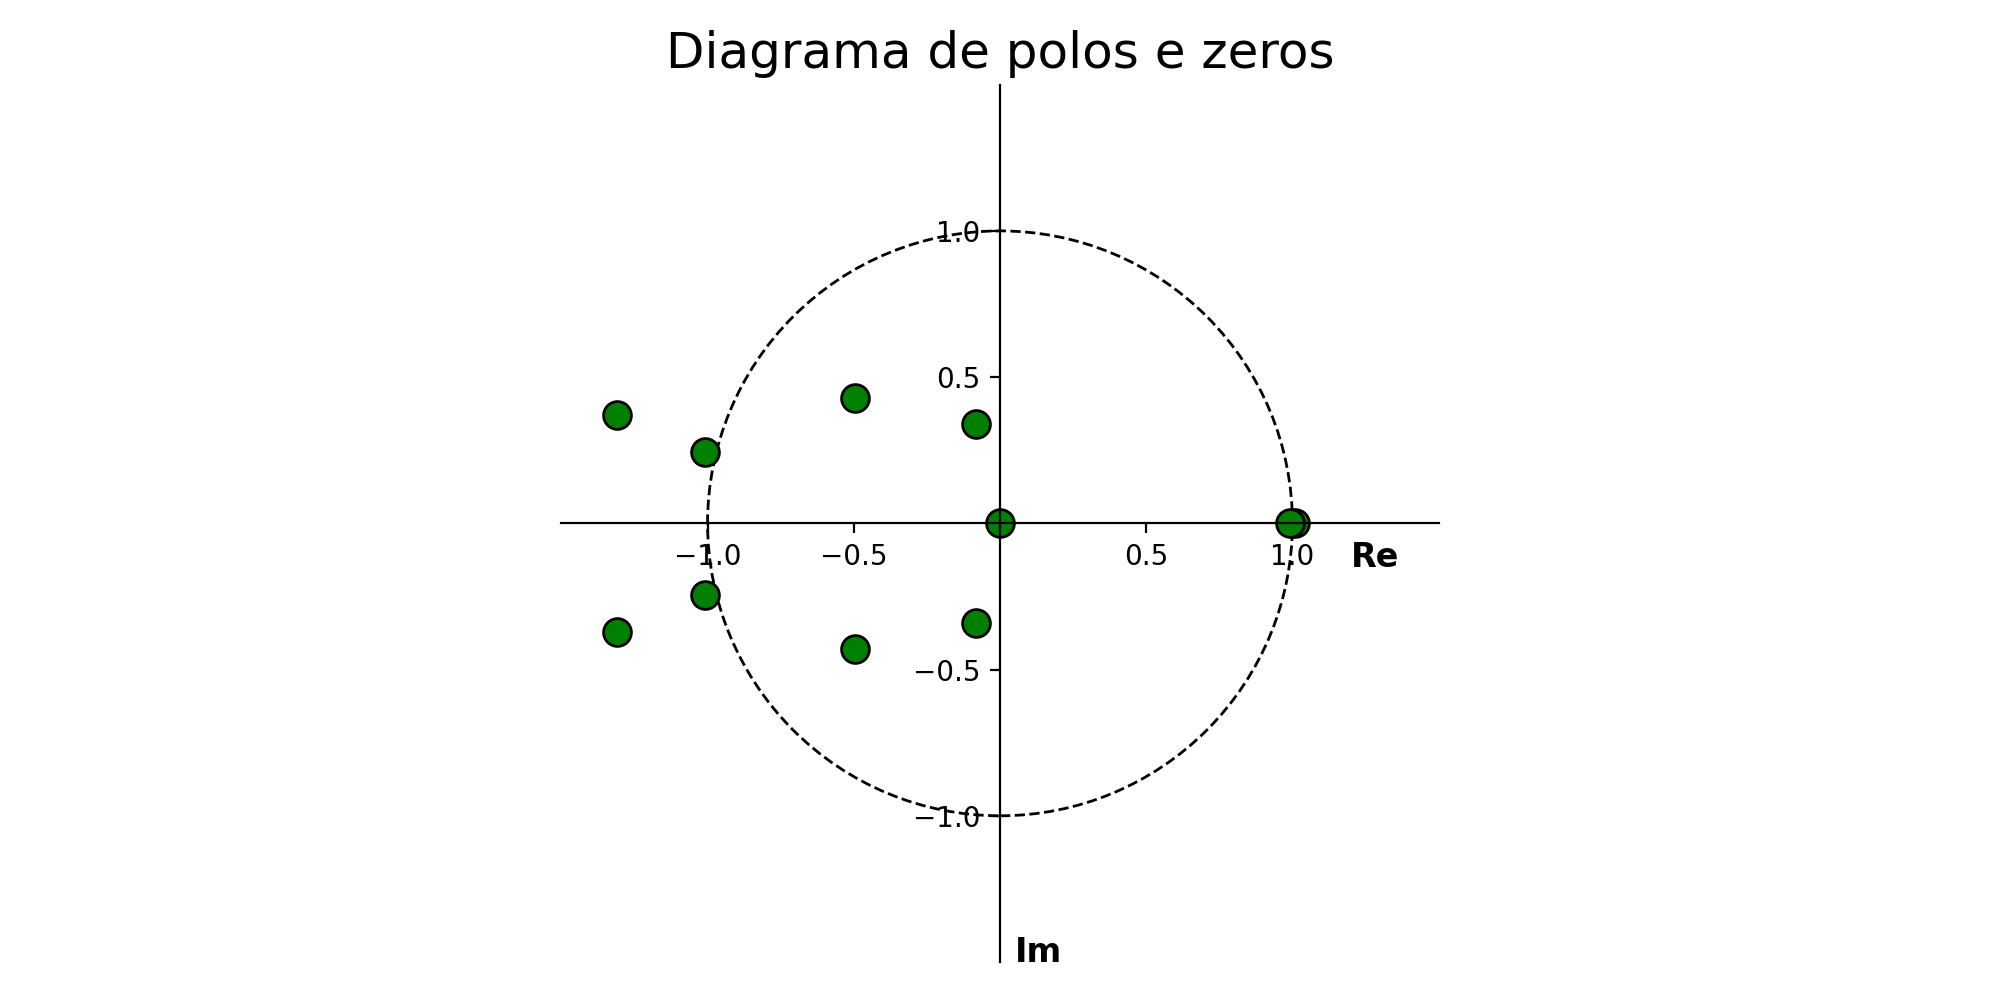
\includegraphics[width=8cm,height=4cm]{Imgs/Metodologia/ricker_zero_phase_b.png}\label{fig:}}
	
	\subfloat[]{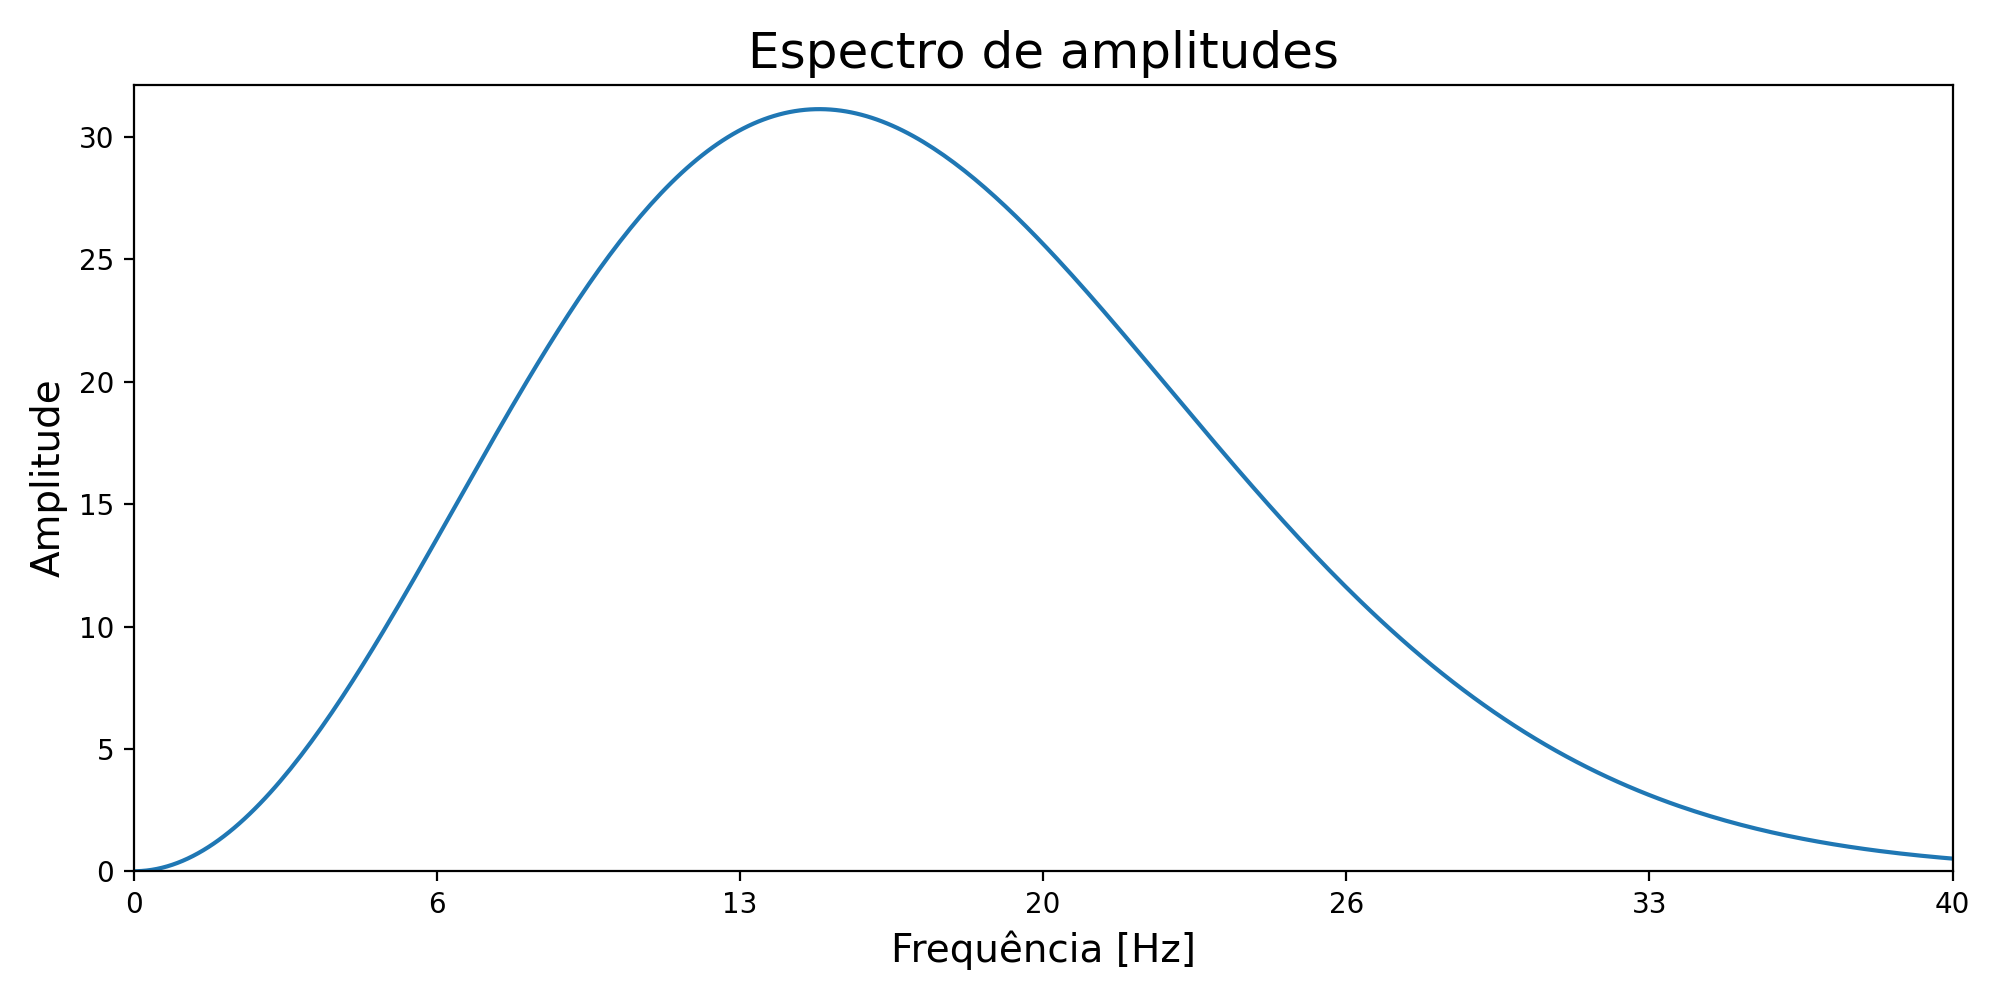
\includegraphics[width=8cm,height=4cm]{Imgs/Metodologia/ricker_zero_phase_c.png}\label{fig:}}
	\subfloat[]{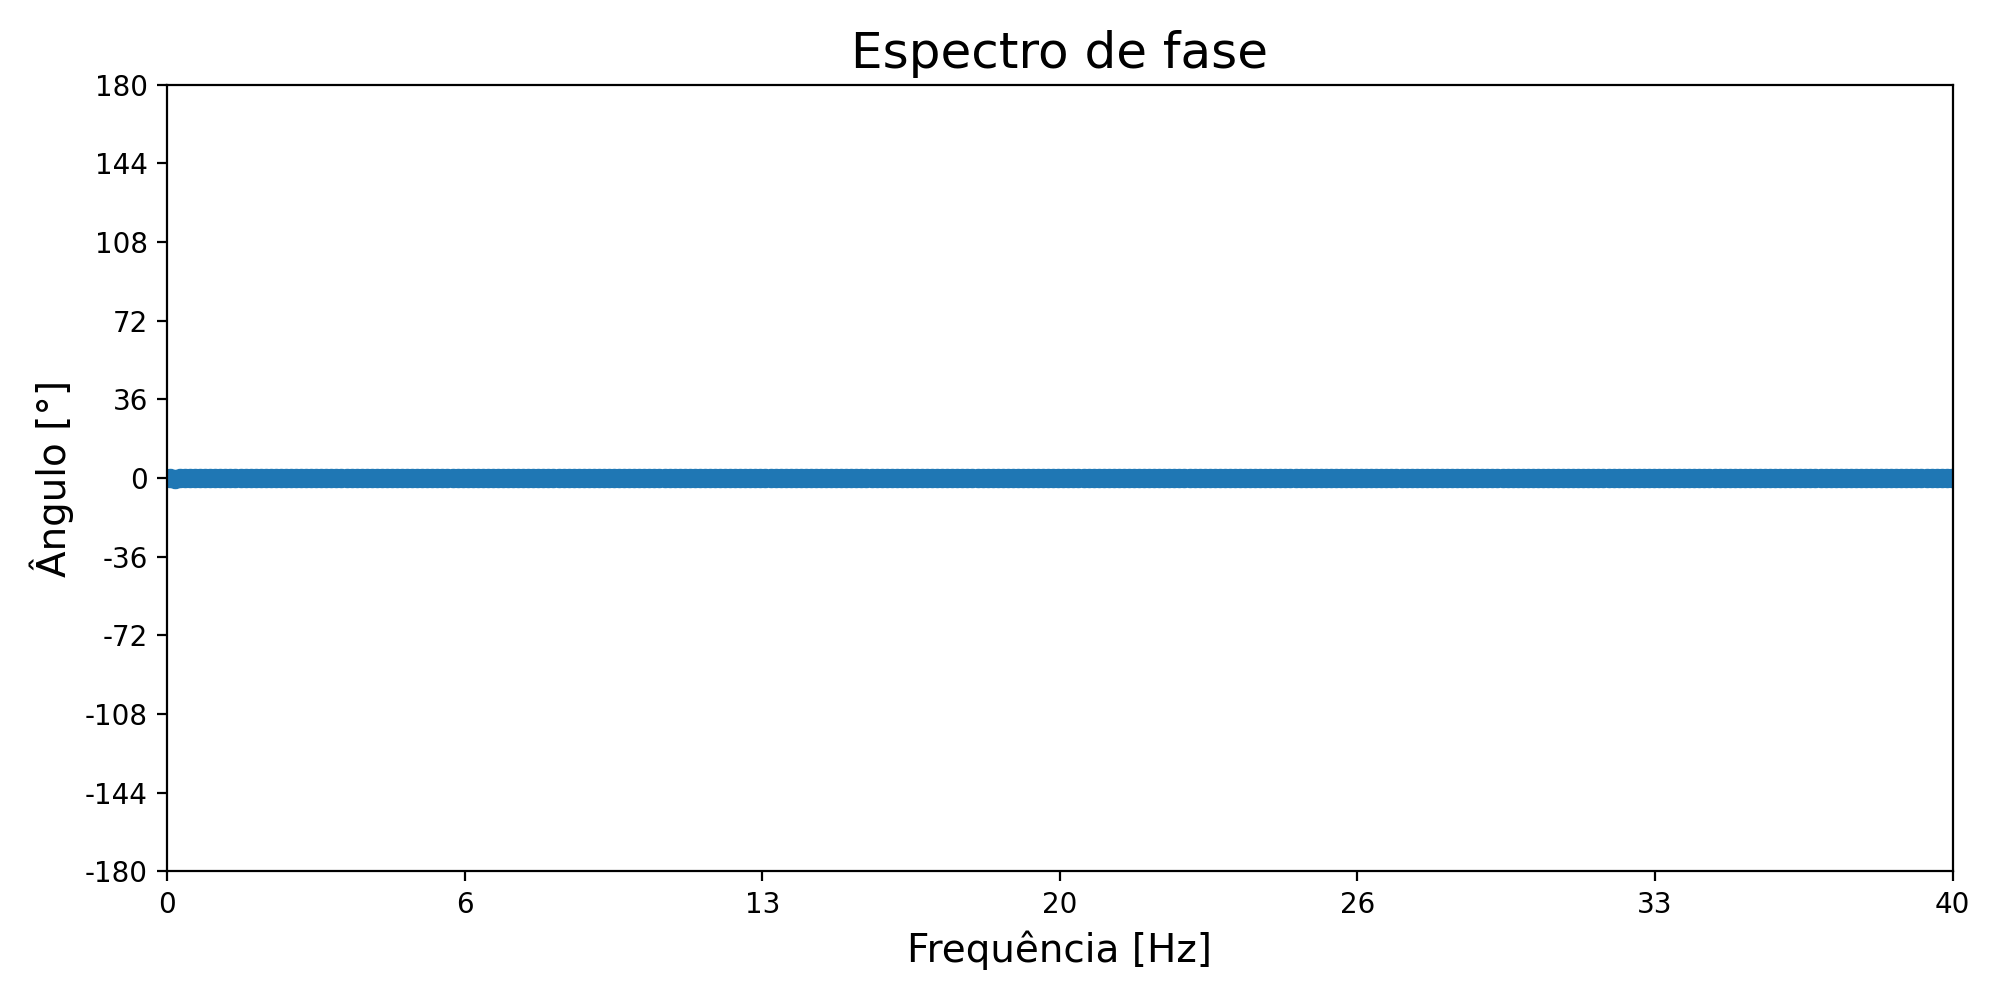
\includegraphics[width=8cm,height=4cm]{Imgs/Metodologia/ricker_zero_phase_d.png}\label{fig:}}
		
	\caption{caption}
	\label{fig:}
\end{figure}



\begin{figure}[H]
	\centering
	\subfloat[]{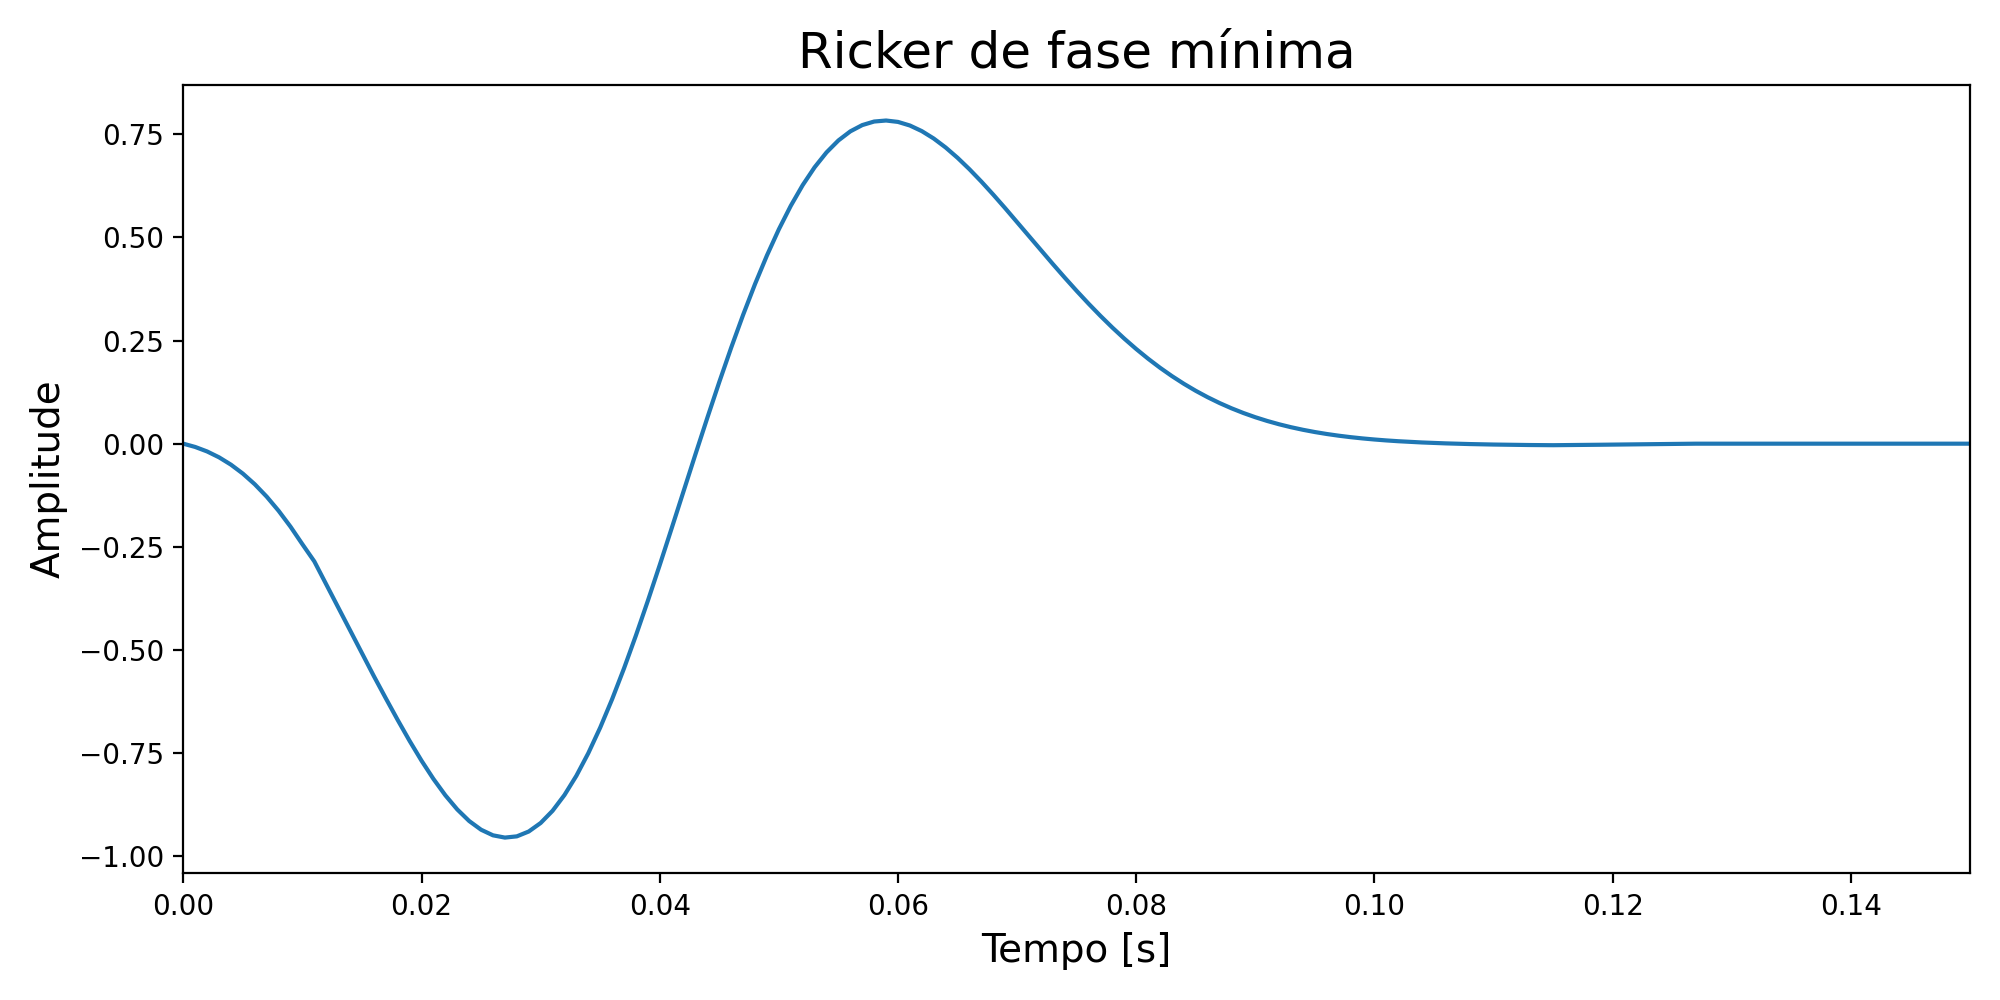
\includegraphics[width=8cm,height=4cm]{Imgs/Metodologia/ricker_min_phase_a.png}\label{fig:}}
	\subfloat[]{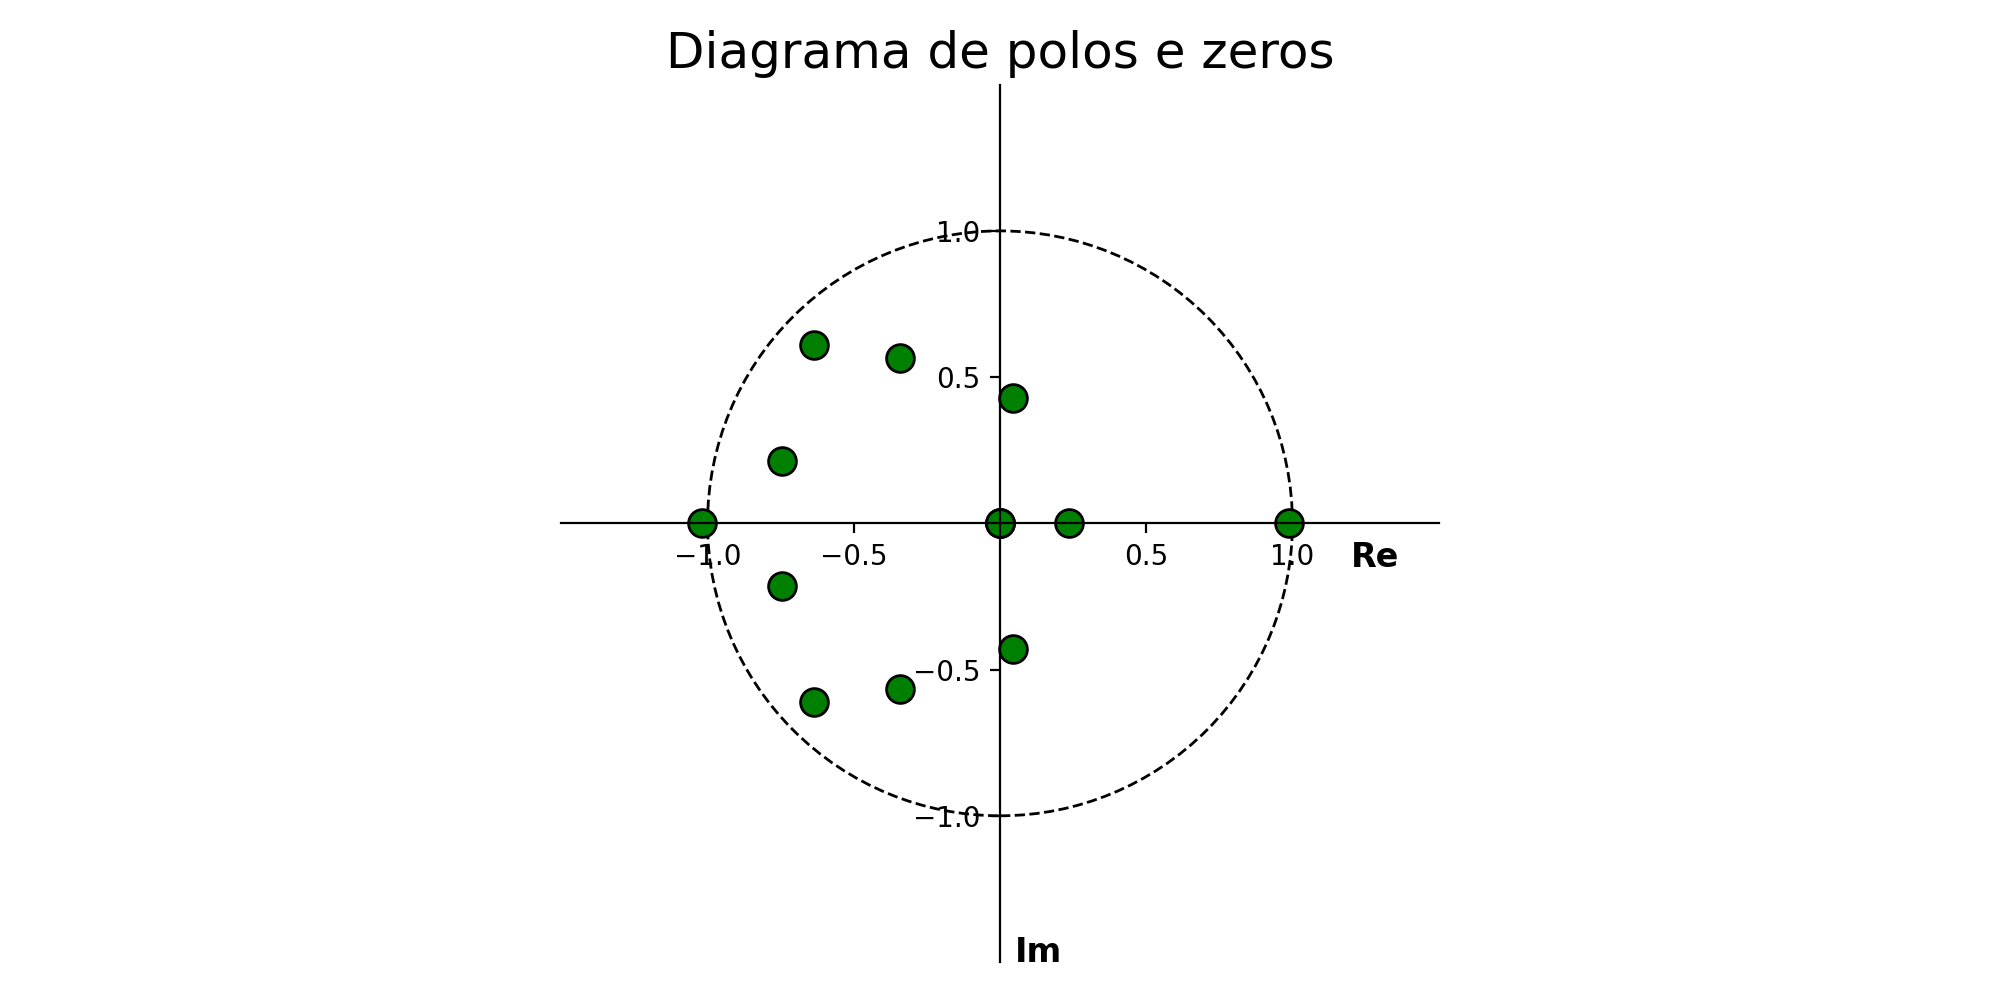
\includegraphics[width=8cm,height=4cm]{Imgs/Metodologia/ricker_min_phase_b.png}\label{fig:}}
	
	\subfloat[]{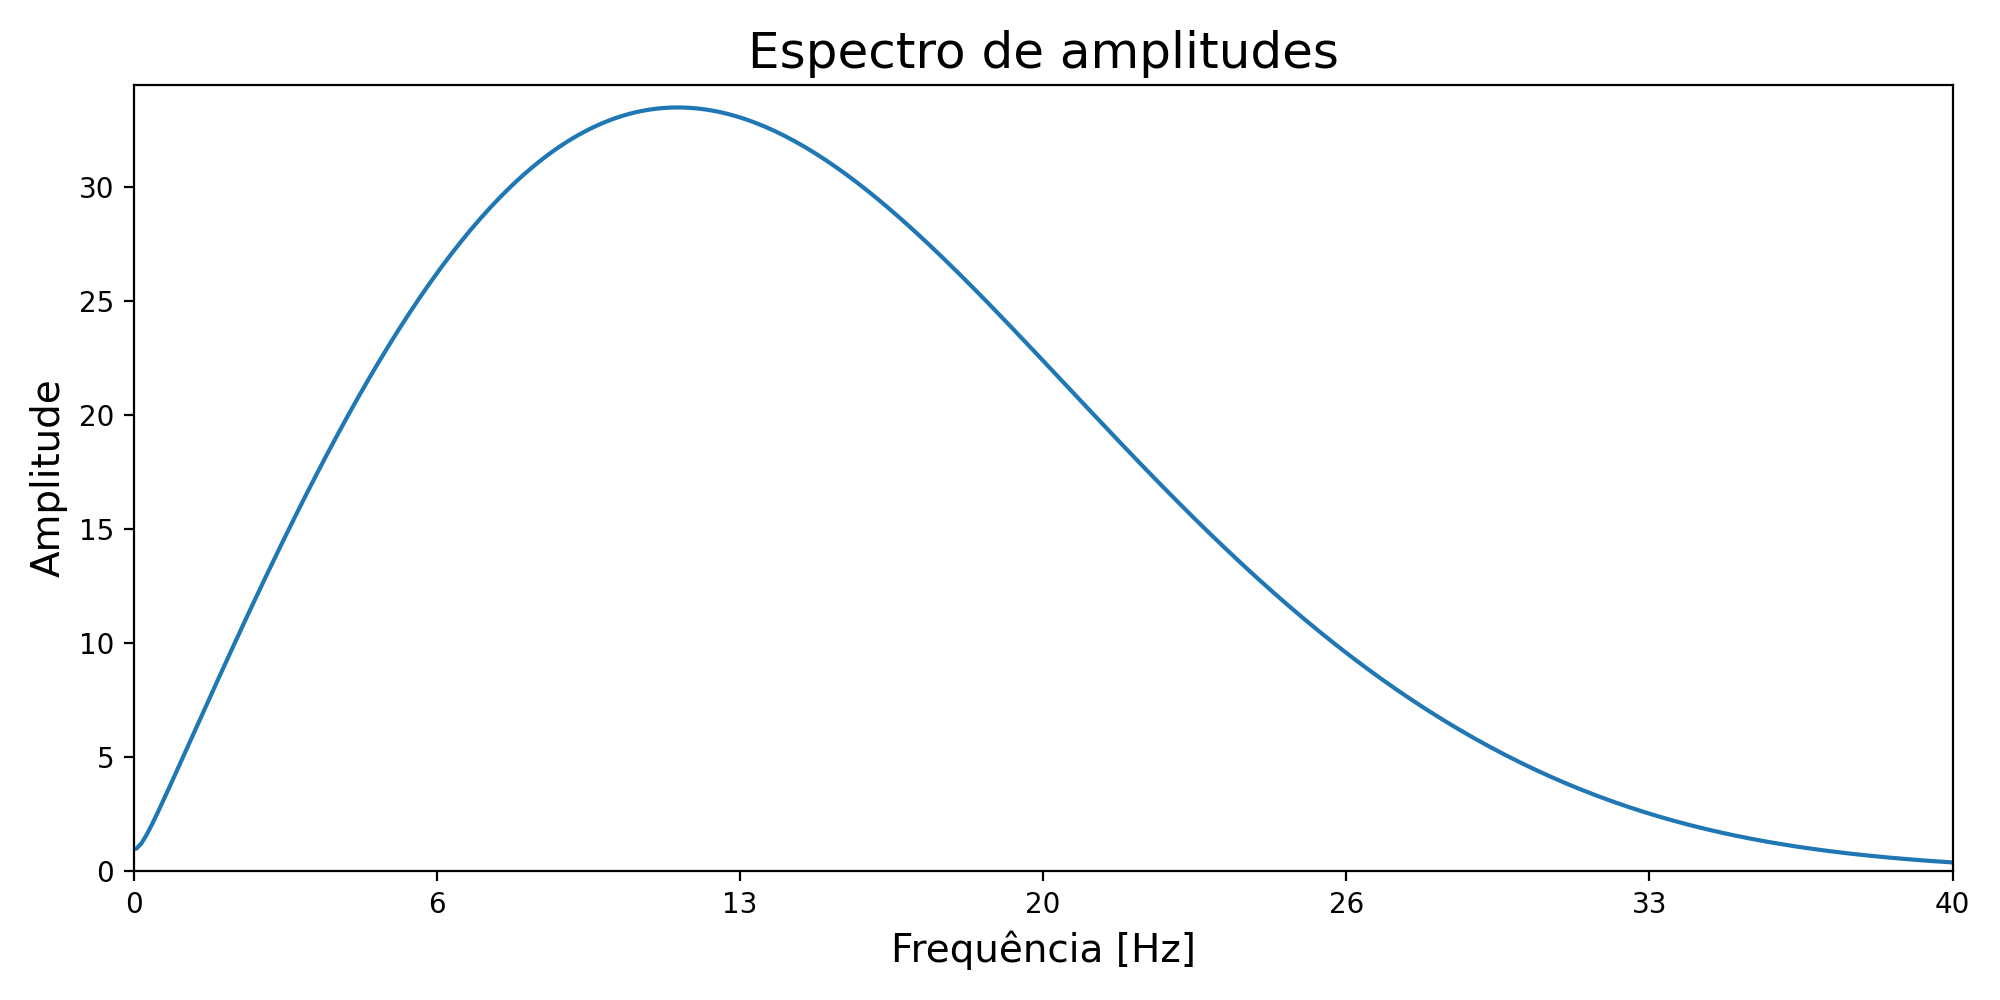
\includegraphics[width=8cm,height=4cm]{Imgs/Metodologia/ricker_min_phase_c.png}\label{fig:}}
	\subfloat[]{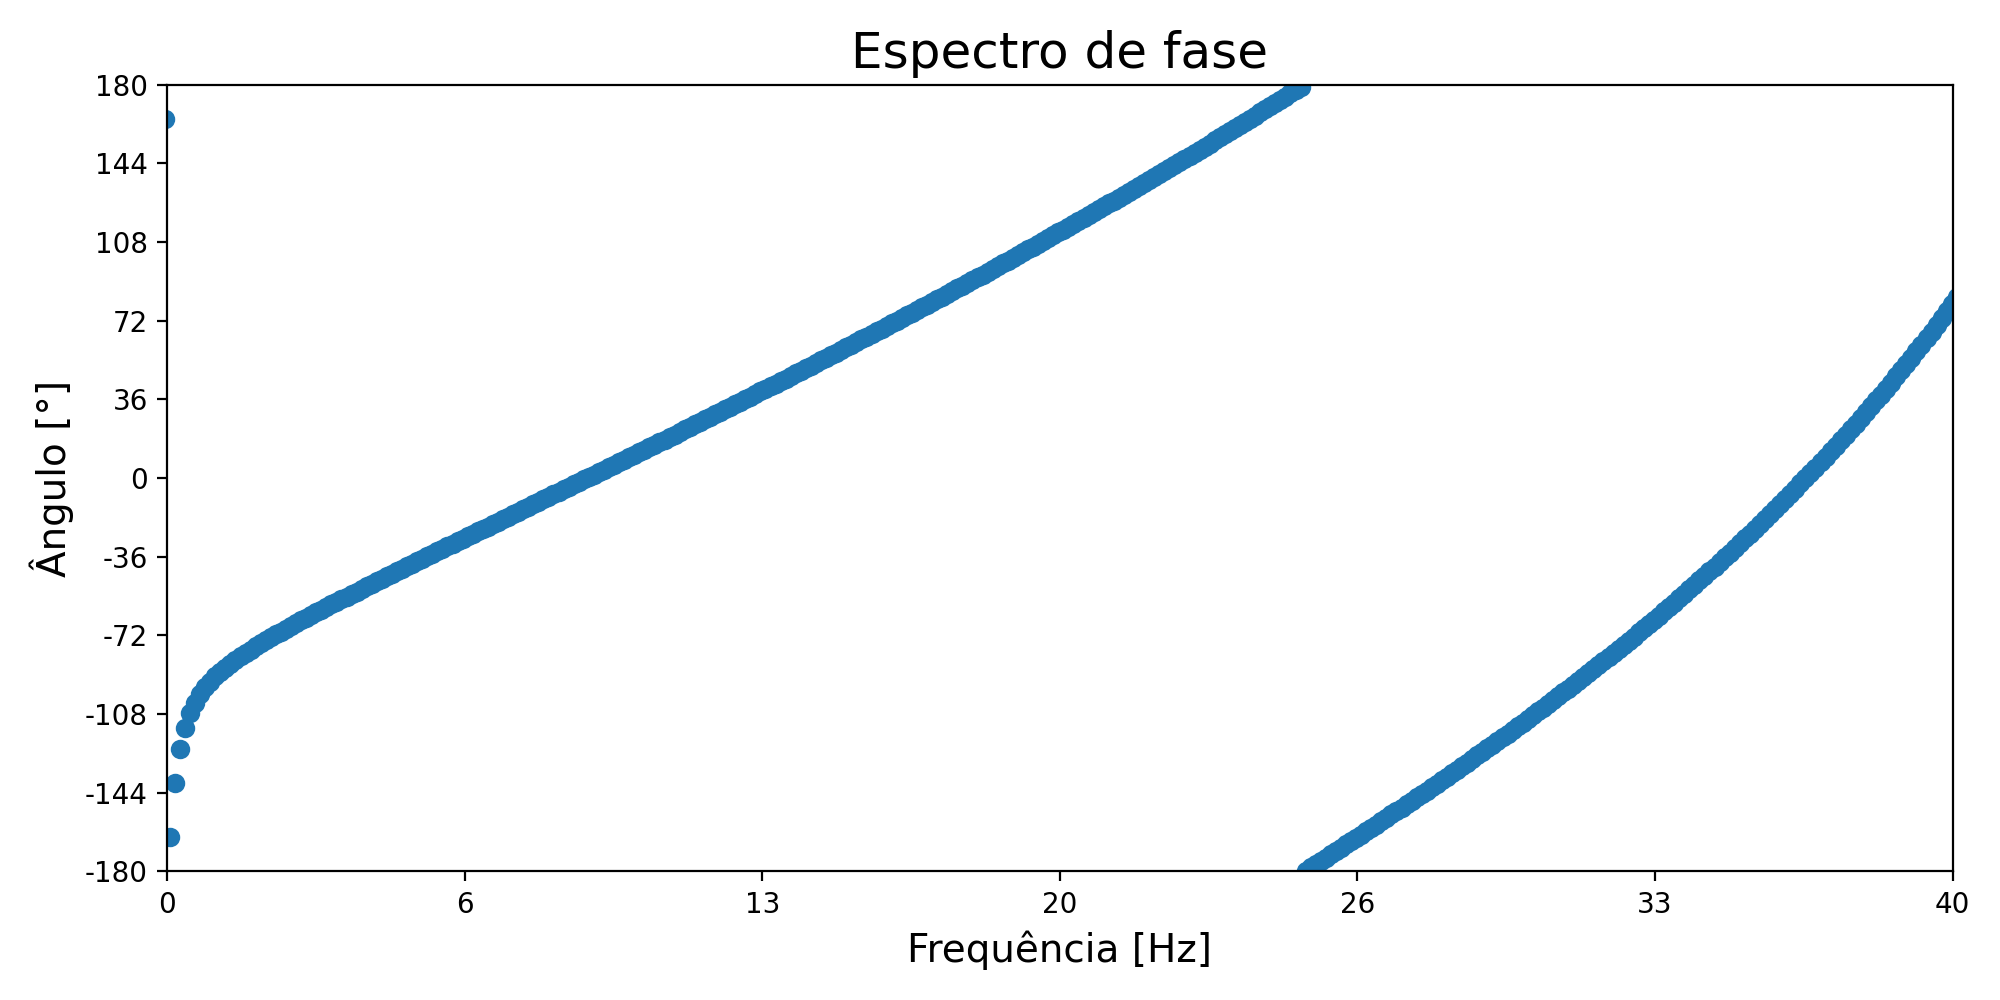
\includegraphics[width=8cm,height=4cm]{Imgs/Metodologia/ricker_min_phase_d.png}\label{fig:}}
	
	\caption{caption}
	\label{fig:}
\end{figure}


\begin{figure}[H]
	\centering
	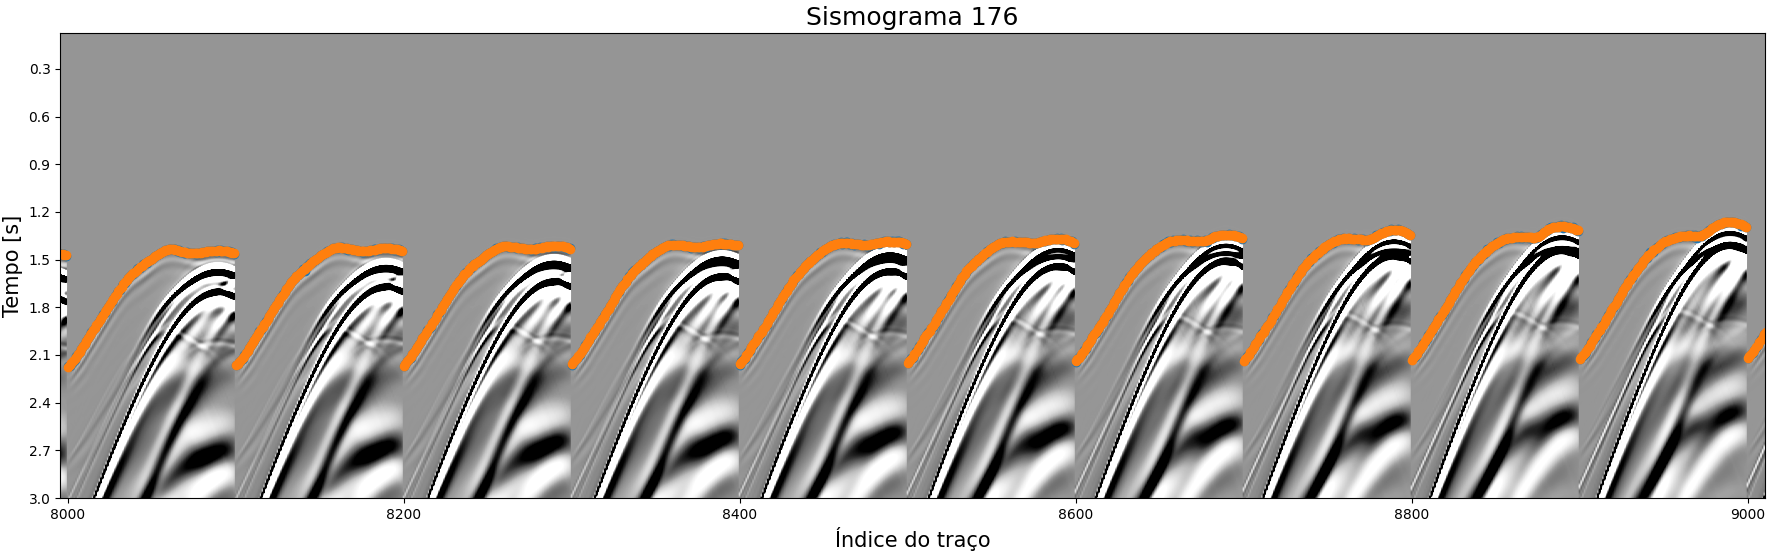
\includegraphics[width=16cm,height=5cm]{Imgs/Metodologia/gather_example.png}
	\caption{caption}
	\label{fig:}	
\end{figure}





\begin{figure}[H]
	\centering
	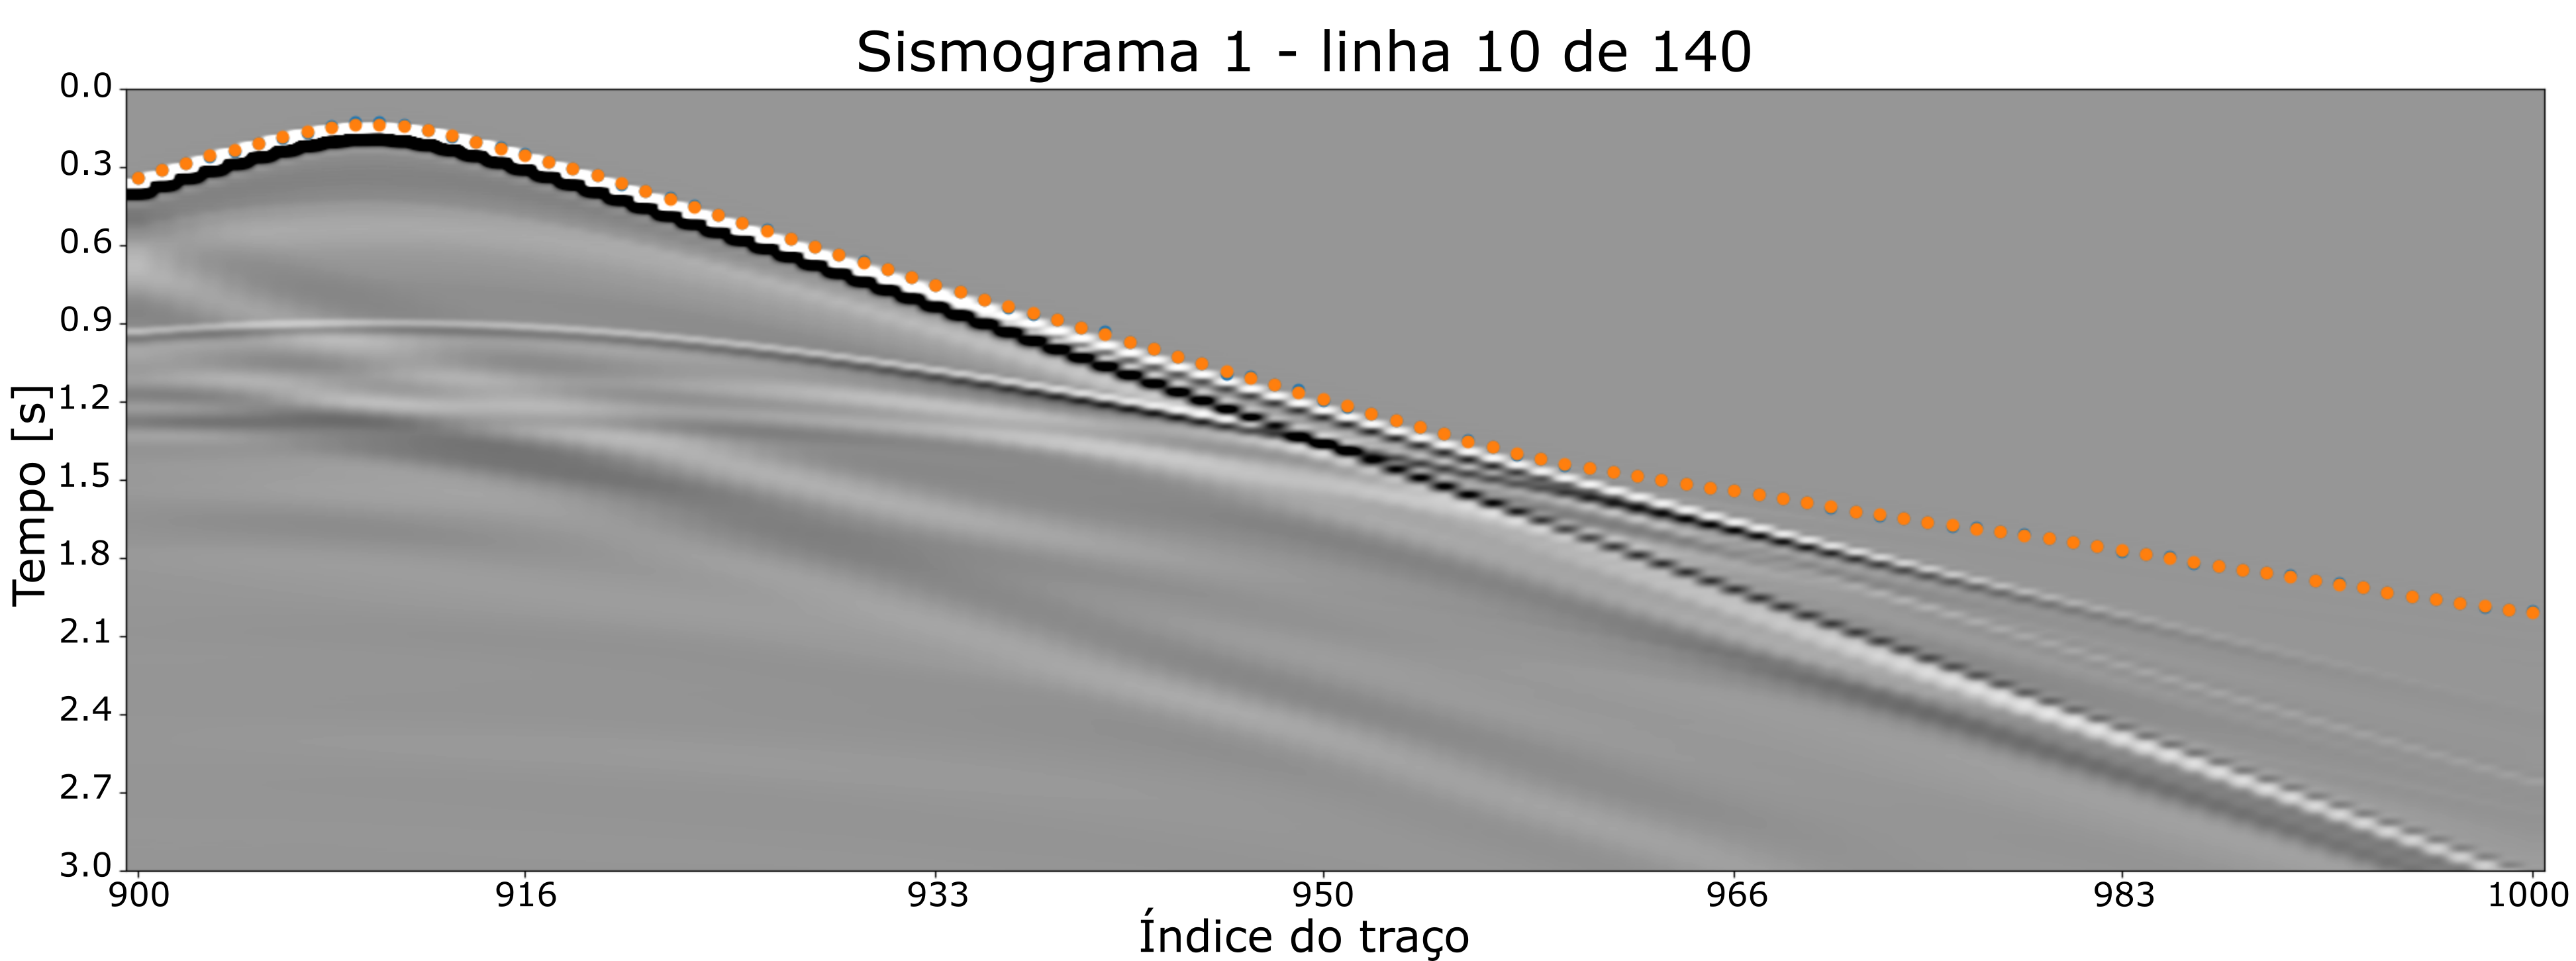
\includegraphics[width=16cm,height=6cm]{Imgs/Metodologia/linha10_sismo1.png}
	\caption{caption}
	\label{fig:}	
\end{figure}

\begin{figure}[H]
	\centering
	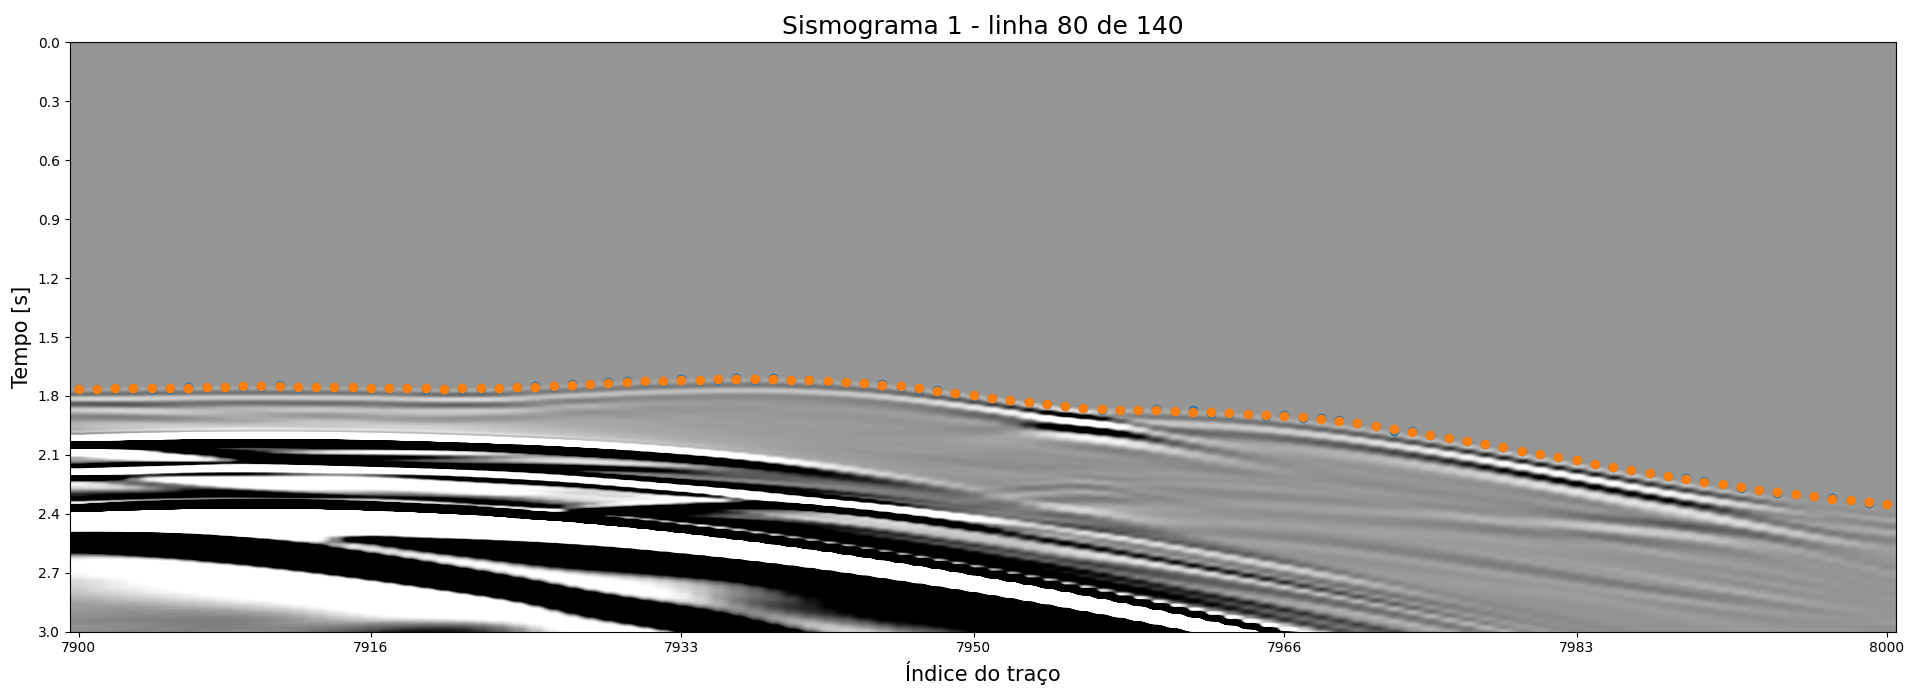
\includegraphics[width=16cm,height=6cm]{Imgs/Metodologia/linha80_sismo1.png}
	\caption{caption}
	\label{fig:}	
\end{figure}

\begin{figure}[H]
	\centering
	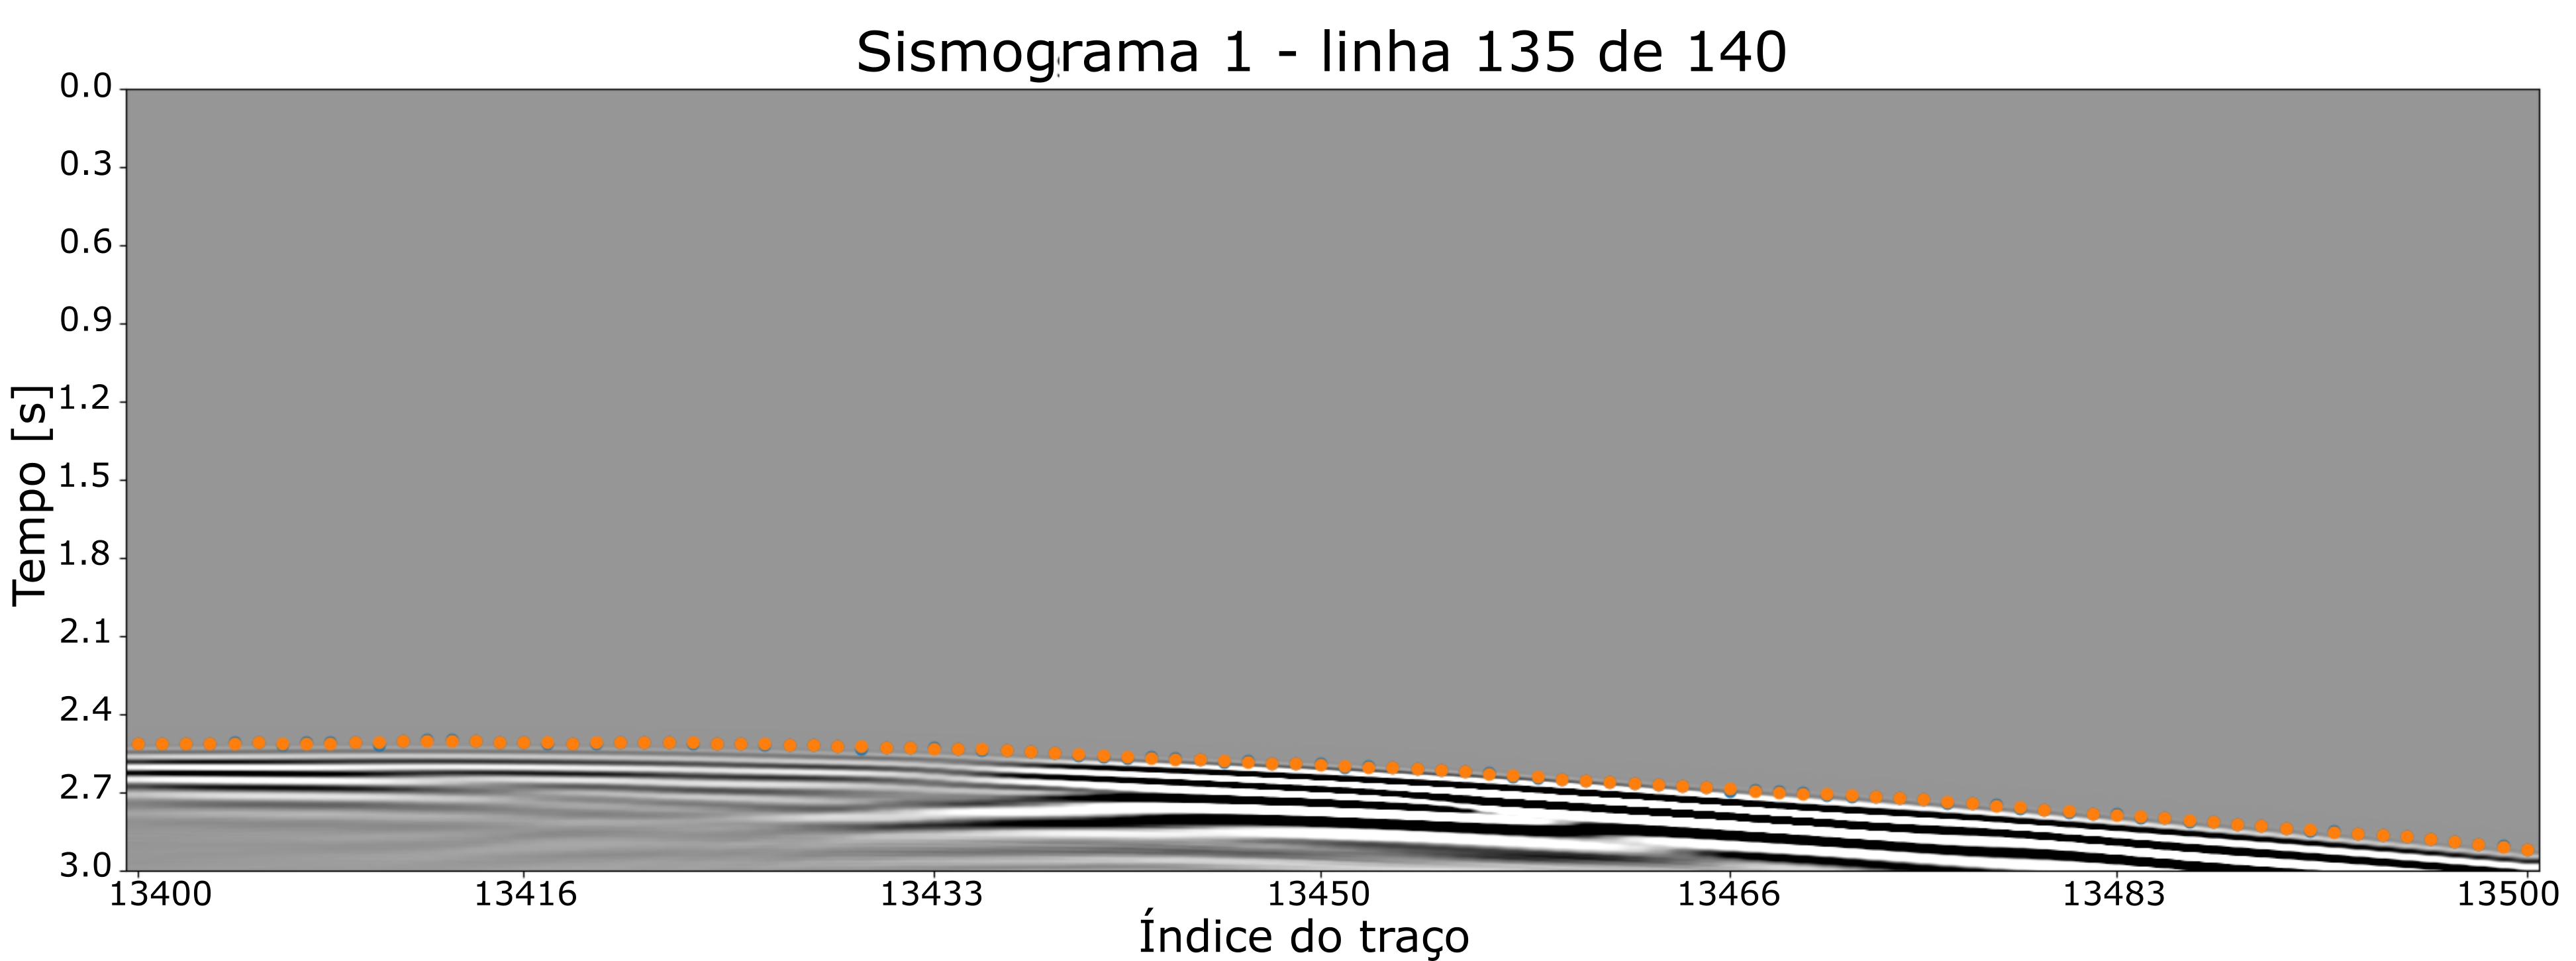
\includegraphics[width=16cm,height=6cm]{Imgs/Metodologia/linha135_sismo1.png}
	\caption{caption}
	\label{fig:}	
\end{figure}




\section{Configurações do esquema de inversão}



